%\documentclass[handout]{beamer}
%\documentclass[handout,10pt,slidestop,mathserif]{beamer}
%\usepackage{pgfpages}
%\pgfpagesuselayout{2 on 1}
\documentclass[10pt,slidestop,mathserif,c]{beamer}
\usetheme{Madrid}
\usecolortheme{seahorse}

\usepackage{tabularx}
\usepackage{verbatim}
\usepackage{graphics}
\usepackage{graphicx}
\usepackage{Sweave}
\usepackage{moreverb}
\usepackage{pgf}
\usepackage{tikz}
\usepackage{Sweave}
%\SweaveOpts{prefix.string=figures/}

\newcommand{\putat}[3]{\begin{picture}(0,0)(0,0)\put(#1,#2){#3}\end{picture}}
  
\newenvironment{changemargin}[2]{%
  \begin{list}{}{%
    \setlength{\topsep}{0pt}%
    \setlength{\leftmargin}{#1}%
    \setlength{\rightmargin}{#2}%
    \setlength{\listparindent}{\parindent}%
    \setlength{\itemindent}{\parindent}%
    \setlength{\parsep}{\parskip}%
  }%
  \item[]}{\end{list}}

%% Define a new 'leo' style for the package that will use a smaller font.
\makeatletter
\def\url@leostyle{%
  \@ifundefined{selectfont}{\def\UrlFont{\sf}}{\def\UrlFont{\tiny\ttfamily}}}
\makeatother

\title{EPSY 887: Computation Statistics}
\subtitle{Introductions}
\author[Jason Bryer]{Jason M. Bryer}
\institute[Jason.Bryer.org]{\url{http://github.com/jbryer/CompStats}\\\href{mailto:jason@bryer.org}{jason@bryer.org}}
\date[Jan 28, 2013]{Week 1\\January 28, 2013}

\begin{document}

\AtBeginSection[]
{
   \begin{frame}
       \frametitle{Outline}
       \tableofcontents[currentsection,currentsubsections]
   \end{frame}
}


\frame{\titlepage}
\frame{\frametitle{Agenda}\tableofcontents[hideallsubsections]}

\section{Introductions}

\begin{frame}[fragile]
	\frametitle{Introductions}
	\begin{itemize}
		\item Your name and department.
		\item Experience with R.
		\item Research interests.
		\item What experiences have you had with larger datasets.
	\end{itemize}

\end{frame}


\section{Course Overview}


\begin{frame}[fragile]
	\frametitle{Why learn to program?}
	\begin{itemize}
	\item<+-| alert@+> \textit{Independence}: otherwise, you rely on someone else always having made exactly the right tool for you, and giving it to you.
	\item<+-| alert@+> \textit{Honesty}: otherwise, you end up distorting the problem to match the tools you happen to have.
	\item<+-| alert@+> \textit{Clarity}: turning your method into something a machine can do forces you to discipline your thinking and make it communicable.
	\end{itemize}
	\vfill
	 \scriptsize (Shalizi, 2012, \url{http://www.stat.cmu.edu/~cshalizi/statcomp/})
\end{frame}

\begin{frame}[fragile]
	\frametitle{Reproducible Research}
	
	\begin{quote}Let us change our traditional attitude to the construction of programs: Instead of imagining that our main task is to instruct a computer what to do, let us concentrate rather on explaining to humans what we want the computer to do.\end{quote}
	\begin{flushright}\scriptsize Knuth, D. E. (1984). Literate Programming. \textit{The Computer Journal, 27}(2):97-111\end{flushright}
	
	
\end{frame}

\begin{frame}[fragile]
	\frametitle{Textbooks}
	\begin{itemize}
		\item Kabacoff, R.J. (2011). \textit{R in Action: Data Analysis and Graphics with R}. Shelter Island, NY: Manning. \\
		\begin{center}
\includegraphics[keepaspectratio,height=80px]{figures/rinaction.jpg}\end{center}
		\item Matloff, N. (2011). \textit{The Art of R Programming}. San Francisco, CA: No Starch Press.\\
		\begin{center}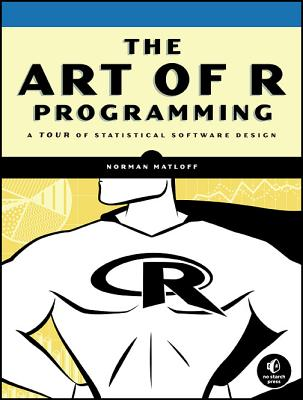
\includegraphics[keepaspectratio,height=80px]{figures/theartofrprogramming.jpg}\end{center}
	\end{itemize}
\end{frame}

\begin{frame}[fragile]
	\frametitle{Topics to Cover During the Semester}
	The following list of topics is subject to change based upon your interest. 
	\begin{itemize}
		\item Using R as a programming language including control statements (including \texttt{if}, \texttt{for}, \texttt{while} statements) and functional programming.
		\item Advanced data visualizations.
		\item Object oriented programming (i.e. S3, S4, and Reference Classes)
		\item Missing data
		\item Analysis of complex survey designs
		\item \LaTeX{}
		\item R package development\\
	\end{itemize}
	\pause
	Other statistical topics including:
	\begin{itemize}
		\item Propensity score analysis
		\item Multilevel modeling (HLM)
		\item Item response theory (IRT)
	\end{itemize}
\end{frame}

\section{Software}

\begin{frame}[fragile,containsverbatim]
	\frametitle{Software}
	We will utilize the following software:
	\begin{itemize}
		\item R (\url{www.r-project.org})
		\item RStudio (\url{www.rstudio.com})
		\item \LaTeX{} (\href{http://tug.org/mactex/}{MacTeX} or \href{http://miktex.org/}{MiKTeX})
		\item Git vis-\`a-vis \url{www.github.com}
			\begin{itemize}
				\item Github for Windows \url{http://windows.github.com/}
				\item Github for Mac \url{http://mac.github.com/}
				\item Tower for Mac \url{http://www.git-tower.com/} \footnote{Students get 50\% off}
			\end{itemize}
	\end{itemize}
\end{frame}

\begin{frame}[fragile,containsverbatim]
	\frametitle{Installing R}
	The latest version of R can be obtained from \url{http://cran.r-project.org}. The current version of R is:
\begin{Schunk}
\begin{Sinput}
> R.version$version.string
\end{Sinput}
\begin{Soutput}
[1] "R version 2.15.2 (2012-10-26)"
\end{Soutput}
\end{Schunk}
	\pause
	\ \\
	For Windows the following should also be installed:
	\begin{itemize}
		\item RTools \url{http://www.murdoch-sutherland.com/Rtools/}
		\item \href{http://downloads.activestate.com/ActivePerl/releases/5.16.1.1601/ActivePerl-5.16.1.1601-MSWin32-x86-296175.msi}{ActivePerl}
	\end{itemize}
	\ \\ \ \\
	For Mac the following should also be installed which are available from \url{http://cran.r-project.org/bin/macosx/tools}
	\begin{itemize}
		\item gfortran-4.2.3
		\item tcl/tk 8.5.5
	\end{itemize}
	\vfill
	Detailed installation instructions are on the course website: \url{https://github.com/jbryer/CompStats/blob/master/Installation/}
\end{frame}


\section{Data}

\begin{frame}[fragile]
	\frametitle{Data Sources}
	
	\begin{itemize}
		\item Programme for International Student Assessment (PISA) 
		\item DataFerrett (Federated Electronic Research, Review, Extraction, and Tabulation Tool)
		\item The World Bank
		\item Trends in International Mathematics and Science Study (TIMSS)
		\item Progress in International Reading Literacy Study (PIRLS)
		\item California Department of Education
		\item School Attendance Boundary Information System (SABINS)
		\item American Community Survey
		\item Integrated Postsecondary Education Data System (IPEDS) Data about higher education institutions. 
		\item Google Public Data
		\item Zanran A search engine for data and statistics.
		\item The Washington Post The Washington Post has compiled a list of some data sources.
		\item Inter-university Consortium for Political and Social Research
	\end{itemize}
\end{frame}

\section{Introduction to R}

\begin{frame}
	\frametitle{What is R?}
	\begin{quote}R is a language and environment for statistical computing and graphics. It is a GNU project which is similar to the S language and environment which was developed at Bell Laboratories (formerly AT\&T, now Lucent Technologies) by John Chambers and colleagues...
	\end{quote}
	\pause
	\begin{quote}
	R provides a wide variety of statistical (linear and non linear modeling, classical statistical tests, time-series analysis, classifcation, clustering, ...) and graphical techniques, and is highly extensible. The S language is often the vehicle of choice for research in statistical methodology, and R provides an Open Source route to participation in that activity.
	(R-project.org)
	\end{quote}
\end{frame}


\begin{frame}[c]
	\frametitle{R's Roots... S}
	\begin{itemize}
	\item S is a language that was developed by John Chambers and others at Bell Labs.
	\item S was initiated in 1976 as an internal statistical analysis environment - originally implemented as Fortran libraries.
	\item Early versions of the language did not contain functions for statistical modeling.
	\item In 1988 the system was rewritten in C and began to resemble the system that we have today (this was Version 3 of the language). The book Statistical Models in S by Chambers and Hastie (the blue book) documents the statistical analysis functionality.
	\item Version 4 of the S language was released in 1998 and is the version we use today. The book Programming with Data by John Chambers (the green book) documents this version of the language.
	\end{itemize}
\end{frame}

\begin{frame}[c]
	\frametitle{History of S}
	\begin{itemize}
	\item In 1993 Bell Labs gave StatSci (now Insightful Corp.) an exclusive license to develop and sell the S language.
	\item In 2004 Insightful purchased the S language from Lucent for \$2 million and is the current owner.
	\item In 2006, Alcatel purchased Lucent Technologies and is now called Alcatel-Lucent.
	\item Insightful sells its implementation of the S language under the product name S-PLUS and has built a number of fancy features (GUIs, mostly) on top of it-hence the "PLUS".
	\item In 2008 Insightful is acquired by TIBCO for \$25 million; future of S-PLUS is uncertain.
	\item The S language itself has not changed dramatically since 1998.
	\item In 1998, S won the Association for Computing Machinery's Software System Award.
	\end{itemize}
\end{frame}

\begin{frame}[c]
In "Stages in the Evolution of S", John Chambers writes:
\begin{quote}
"[W]e wanted users to be able to begin in an interactive environment, where they did not consciously think of themselves as programming. Then as their needs became clearer and their sophistication increased, they should be able to slide gradually into programming, when the language and system aspects would become more important."
\end{quote}
http://www.stat.bell-labs.com/S/history.html
\end{frame}

\begin{frame}[c]
	\frametitle{History of R}
	\begin{itemize}
	\item 1991: Created in New Zealand by Ross Ihaka and Robert Gentleman. Their experience developing R is documented in a 1996 JCGS paper.
	\item 1993: First announcement of R to the public.
	\item 1995: Martin Machler convinces Ross and Robert to use the GNU General Public License to make R free software.
	\item 1996: A public mailing list is created (R-help and R-devel)
	\item 1997: The R Core Group is formed (containing some people associated with S-PLUS). The core group controls the source code for R.
	\item 2000: R version 1.0.0 is released.
	\item 2012: R version 2.15.2 is released on October 31, 2012.
	\item There are now over 4,000 packages listed on CRAN. 
	\end{itemize}
\end{frame}

\begin{frame}[containsverbatim,fragile]
	\frametitle{R as a Big Calculator}
	\setbeamercovered{invisible}
\begin{Schunk}
\begin{Sinput}
> 2 + 2
\end{Sinput}
\begin{Soutput}
[1] 4
\end{Soutput}
\end{Schunk}
\pause
\begin{Schunk}
\begin{Sinput}
> 1 + sin(9)
\end{Sinput}
\begin{Soutput}
[1] 1.4
\end{Soutput}
\end{Schunk}
\pause
\begin{Schunk}
\begin{Sinput}
> 23.76 * log(8)/(23+atan(9))
\end{Sinput}
\begin{Soutput}
[1] 2
\end{Soutput}
\end{Schunk}
\end{frame}

\begin{frame}[containsverbatim]
	\frametitle{Installing Packages}
	Both Windows and Mac have a menu system for installing packages, however the \texttt{install.packages} function allows for the installation to be scriptable.
\begin{Schunk}
\begin{Sinput}
> install.packages(c("psych", "gdata", "foreign", "devtools", 
   "roxygen"), dependencies = TRUE)
\end{Sinput}
\end{Schunk}
\vfill
See the \texttt{Setup.r} script for more details, including some special details for installing some packages on Windows (e.g. \texttt{XML} package).
\vfill
We will also install packages that are not yet on CRAN but are on Github. The \texttt{install\_github} function in the \texttt{devtools} package allows us to install those packages:
\begin{Schunk}
\begin{Sinput}
> require(devtools)
> install_github("pisa","jbryer")
\end{Sinput}
\end{Schunk}

\end{frame}

\begin{frame}[containsverbatim,fragile]
	\frametitle{Loading Packages}
	\setbeamercovered{invisible}
	The \texttt{require} command\footnote{The \texttt{library} command will also load packages but the \texttt{require} is now preferred.} will load a package into the current R session.
\begin{Schunk}
\begin{Sinput}
> require(psych)
> require(gdata)
> require(foreign)
\end{Sinput}
\end{Schunk}
	\pause
	\vfill
	For a list of packages that have been downloaded, but not necessarily attached, the \texttt{library()} function without any parameters will return that list.
\begin{Schunk}
\begin{Sinput}
> library()
\end{Sinput}
\end{Schunk}
\end{frame}

\begin{frame}[containsverbatim,fragile]
	\frametitle{Getting Help}
	\begin{itemize}
	\item<+-| alert@+>{ R provides extensive documentation and help. The \texttt{help.start()} function will launch a webpage with links to:
	\begin{itemize}
		\item The R manuals
		\item The R FAQ
		\item Search engine
		\item and many other useful sites
	\end{itemize} }
	\item<+-| alert@+>{ The \texttt{help.search()} function will search the help file for a particular word or phrase. For example:
\begin{Schunk}
\begin{Sinput}
> help.search("cross tabs")
\end{Sinput}
\end{Schunk}
}
	\item<+-| alert@+>{ To get documentation on a specific function, the \texttt{help()} function, or simply \texttt{?functionName} will open the documentation page in the web browser.}
	\item<+-| alert@+>{ Lastly, to search the R mailing lists, use the \texttt{RSiteSearch()} function.}
	\end{itemize}
\end{frame}

\begin{frame}[fragile]
	\frametitle{NA vs. NULL}
	\setbeamercovered{invisible}
	R is just as much a programming language as it is a statistical software package. As such it represents null differently for programming (using NULL) than for data (using NA).
	\pause
	\begin{quote}NULL represents the null object in R: it is a reserved word. NULL is often returned by expressions and functions whose values are undefined.	\end{quote}	
	\pause
	\begin{quote}NA is a logical constant of length 1 which contains a missing value indicator. NA can be freely coerced to any other vector type except raw. There are also constants NA\textunderscore integer\textunderscore, NA\textunderscore real\textunderscore, NA\textunderscore complex\textunderscore and NA\textunderscore character\textunderscore of the other atomic vector types which support missing values: all of these are reserved words in the R language.\end{quote}
	For more details, see~\url{http://opendatagroup.com/2010/04/25/r-na-v-null/}
\end{frame}


\begin{frame}[fragile,containsverbatim]
	\frametitle{Atomic Vectors}
	R has six atomic vectors, they are:
	\begin{itemize}
		\item \texttt{character}
		\item \texttt{numeric}
		\item \texttt{integer}
		\item \texttt{logical}
		\item \texttt{complex}
		\item \texttt{raw}
	\end{itemize}
	\pause
	Methods useful for working with vectors:
	\begin{description}
		\item[\texttt{c}] Concatenate (i.e. combine values into a vector or list)
		\item[\texttt{str}] Provides the structure of any R object (perhaps the most useful function in R!)
		\item[\texttt{names}] Returns the names of an object
		\item[\texttt{dim}] Dimensions of the object
		\item[\texttt{dimnames}] Name of rows and columns of a matrix
		\item[\texttt{class}] Returns the class, or type, of an object
	\end{description}
\end{frame}

\begin{frame}[fragile,containsverbatim]
	\frametitle{Lists}
	Lists are generic vectors where each element can be any R object, including other Lists!
\begin{Schunk}
\begin{Sinput}
> mylist <- list(letters=letters, numbers=1:10)
> class(mylist)
\end{Sinput}
\begin{Soutput}
[1] "list"
\end{Soutput}
\begin{Sinput}
> str(mylist)
\end{Sinput}
\begin{Soutput}
List of 2
 $ letters: chr [1:26] "a" "b" "c" "d" ...
 $ numbers: int [1:10] 1 2 3 4 5 6 7 8 9 10
\end{Soutput}
\begin{Sinput}
> length(mylist)
\end{Sinput}
\begin{Soutput}
[1] 2
\end{Soutput}
\end{Schunk}
\end{frame}

\begin{frame}[fragile,containsverbatim]
	\frametitle{Subsetting Lists and Vectors}
\begin{Schunk}
\begin{Sinput}
> mylist[1]
\end{Sinput}
\begin{Soutput}
$letters
 [1] "a" "b" "c" "d" "e" "f" "g" "h" "i" "j" "k"
[12] "l" "m" "n" "o" "p" "q" "r" "s" "t" "u" "v"
[23] "w" "x" "y" "z"
\end{Soutput}
\begin{Sinput}
> mylist[[1]]
\end{Sinput}
\begin{Soutput}
 [1] "a" "b" "c" "d" "e" "f" "g" "h" "i" "j" "k"
[12] "l" "m" "n" "o" "p" "q" "r" "s" "t" "u" "v"
[23] "w" "x" "y" "z"
\end{Soutput}
\begin{Sinput}
> mylist$letters
\end{Sinput}
\begin{Soutput}
 [1] "a" "b" "c" "d" "e" "f" "g" "h" "i" "j" "k"
[12] "l" "m" "n" "o" "p" "q" "r" "s" "t" "u" "v"
[23] "w" "x" "y" "z"
\end{Soutput}
\begin{Sinput}
> mylist$numbers
\end{Sinput}
\begin{Soutput}
 [1]  1  2  3  4  5  6  7  8  9 10
\end{Soutput}
\end{Schunk}
\end{frame}

\begin{frame}[fragile]
	\frametitle{Reading Data}
	\begin{description}
		\item[read.table] Reads in a table where each line is a record. Lots of options to define the structure of the file.
		\item[read.csv] Comma deliminited files.
		\item[read.spss] In the \texttt{foreign} package, reads SPSS files.
		\item[read.xls] In the \texttt{gdata} package, reads Excel files.
		\item[RODBC] This package has functions to read data from most ODBC databases.
		\item[RMySQL] Package for reading data from MySQL databases.
		\item[RPoostgreSQL] Package for reading data from PostgreSQL databases.
		\item[load] Read in R data object files saved using the \texttt{save}. This is very useful for saving intermediate data files.
	\end{description}
\end{frame}

\begin{frame}[fragile]
	\frametitle{Descriptive Statistics}
	\begin{description}
		\item[table] Crosstabs.
		\item[summary] Provides summary information relevant to the type.
		\item[describe] In the \texttt{psych}, provides many of the most common descriptives statistics (e.g. mean, median, standard deviation, range, etc.)
		\item[describeBy] Same as \texttt{describe} but will provide descriptive stats based upon grouping varaible(s).
		\item[fivenum] Returns Tukey's five number summary (minimum, lower-hinge, median, upper-hinge, maximum)
		\item[mean] Mean
		\item[median] Median
		\item[sd] Standard deviation
		\item[var] Variance
	\end{description}

\end{frame}

%\begin{frame}[c]
%	\LARGE{Thank You}\\
%	\normalsize
%	Jason Bryer (jason@bryer.org)\\
%	\url{http://jbryer.github.com}
%\end{frame}

\end{document}
